\chapter{计算机网络概述}

本章按课件的六部分展开：计算机网络基本概念、计算机网络结构、数据交换、计算机网络性能指标、计算机网络体系结构和计算机网络发展历史。课件第1.6节标注“略”；仍按课件保留其时间线，便于识别重要里程碑。本章中速率、设备和网络结构均以课件所列内容为准。

\section{计算机网络基本概念}

\subsection{通信系统与计算机网络}

计算机网络是通信技术与计算机技术结合的产物。课件给出的通信系统模型由\textbf{信源、发送设备、信道、接收设备、信宿}组成，并可能受到\textbf{噪声源}干扰：
\[
\text{信源}\longrightarrow\text{发送设备}\longrightarrow\text{信道}\longrightarrow\text{接收设备}\longrightarrow\text{信宿}.
\]
信源产生待传送的信息；发送设备把信息变成适合信道传送的信号；信道是信号经过的媒介；接收设备从信号中恢复信息；信宿是信息的最终使用方。噪声是对传输信号的干扰，可能使接收方得到错误信息。

\textbf{计算机网络}是\textbf{互连的、自治的计算机集合}。“互连”表示计算机之间能够借助通信链路交换数据；“自治”表示各计算机没有主从关系，每台计算机仍由自身控制。网络中的计算机通常称为\textbf{主机}或\textbf{端系统}。当距离远、计算机数量多时，不能给每两台计算机都单独铺设一条链路，因此需要交换设备组成交换网络。

\textbf{互联网（Internet）}是由大量互连的计算设备、通信链路和交换设备组成的网络。主机运行网络应用；光纤、铜缆、无线电和卫星等可作为通信链路；路由器和交换机按网络规则转送数据。课件还从服务角度说明，Internet为Web、电子邮件、网络游戏等应用提供通信基础设施和应用编程接口（API）。API是应用程序调用网络功能、连接并收发数据时使用的软件接口。

\textbf{参考书补充：}参考书区分小写的\textit{internet}（多个网络互连而成的通用概念）与大写的\textit{Internet}（特指当前全球最大的互联网络，并使用TCP/IP协议族）。课件主要讨论后者，没有展开这一大小写术语差别。

\begin{figure}[H]
  \centering
  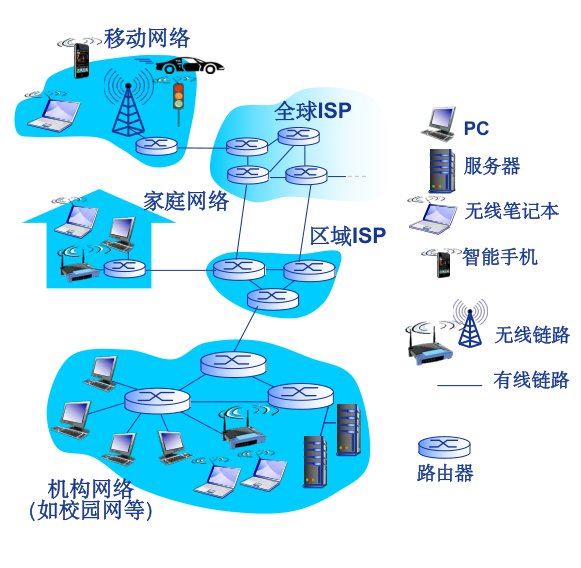
\includegraphics[width=0.82\textwidth]{ch01-internet.png}
  \caption{Internet的组成与互连关系。图中端系统连接家庭、机构、移动和ISP网络；ISP即互联网服务提供商。阅读时可沿链路观察端系统怎样经接入网络进入网络之网络。来源：\texttt{Chapter1-计算机网络概述.pdf}，PDF第8页（课件显示页8），局部截取。}
  \label{fig:ch01-internet}
\end{figure}

\begin{quote}\small\textbf{来源：}课件\texttt{Chapter1-计算机网络概述.pdf}，PDF第4--9页（课件显示页4--9）；参考书第1章§1.1.1--§1.1.3，PDF第12--14页／印刷第1--3页。\end{quote}
\annotationarea[4]

\subsection{网络协议及其三要素}

只把主机、路由器和链路连接起来，不能保证网络应用数据能够按预期交换。网络中的通信实体必须遵循事先约定的规则。\textbf{网络协议}是为网络中的数据交换建立的规则、标准或约定；协议规定通信实体所交换消息的\textbf{格式、含义、顺序}，以及收到消息或发生事件后应采取的动作。

课件把协议要素分为三项：
\begin{itemize}
  \item \textbf{语法（Syntax）}：数据和控制信息的结构或格式，也包括信号电平等表示约定。它回答“消息长什么样”。
  \item \textbf{语义（Semantics）}：控制信息的含义，以及通信实体要执行的动作、响应和差错控制。它回答“收到这条消息应做什么”。
  \item \textbf{时序（Timing）}：事件发生的顺序和速度匹配。它回答“何时发送、先后如何”。
\end{itemize}

课件列出的协议实例包括\textbf{TCP（Transmission Control Protocol，传输控制协议）}、\textbf{IP（Internet Protocol，网际协议）}、\textbf{HTTP（Hypertext Transfer Protocol，超文本传输协议）}和\textbf{802.11无线局域网标准}。Internet标准常通过\textbf{RFC（Request for Comments，请求评论）}文档发布；\textbf{IETF（Internet Engineering Task Force，互联网工程任务组）}参与制定Internet相关标准。RFC是文档系列的名称，不表示每份RFC都是强制标准。

\textbf{区分协议与设备：}设备和链路提供通信的物质基础；协议给通信实体规定交换消息的共同规则。只有链路而没有一致的格式、动作和时序约定，双方就不能可靠地解释收到的数据。

\begin{quote}\small\textbf{来源：}课件\texttt{Chapter1-计算机网络概述.pdf}，PDF第10--16页（课件显示页10--16）；参考书第1章§1.1.2，PDF第13页／印刷第2页。\end{quote}
\annotationarea[4]

\subsection{计算机网络的分类}

课件按三个不同角度分类。它们回答的问题不同，不能把一种角度的类别与另一种角度混为一谈。

\begin{center}
\begin{tabularx}{0.96\textwidth}{l l X}
\toprule
分类角度 & 类别 & 课件给出的含义或范围\\
\midrule
覆盖范围 & PAN（个人区域网） & 约10米\\
 & LAN（局域网） & 约1公里\\
 & MAN（城域网） & 约5--50公里\\
 & WAN（广域网） & 约几十至几千公里\\
使用者 & 专用网（private network） & 供特定组织或用户使用\\
 & 公用网（public network） & 向公众提供网络服务\\
拓扑结构 & 总线、星形、树形、网状 & 描述设备或链路的连接形态\\
\bottomrule
\end{tabularx}
\end{center}

PAN、LAN、MAN、WAN是按覆盖范围划分的网络类别；专用网、公用网按使用者划分；总线、星形、树形、网状按拓扑结构划分。表中距离是课件给出的近似范围，不是所有网络都必须满足的硬性界限。

\begin{quote}\small\textbf{来源：}课件\texttt{Chapter1-计算机网络概述.pdf}，PDF第17页（课件显示页17）。\end{quote}
\annotationarea[4]

\section{计算机网络结构}

\subsection{网络边缘、接入网络与网络核心}

课件把网络结构分成三部分：
\begin{itemize}
  \item \textbf{网络边缘}：主机及其运行的网络应用。用户通过端系统上的应用产生或接收数据。
  \item \textbf{接入网络}：把网络边缘连接到边缘路由器的网络及其物理介质。接入可以使用有线或无线通信链路。
  \item \textbf{网络核心}：互联的路由器或其他分组转发设备构成的网络之网络，负责把数据从源端送往目的端。
\end{itemize}

\textbf{主机}是运行网络应用的端系统。课件介绍两种应用模型：
\begin{itemize}
  \item \textbf{客户/服务器（client/server，C/S）}：客户发送请求，服务器接收请求并返回响应。Web和FTP（File Transfer Protocol，文件传输协议）是课件列出的例子。
  \item \textbf{对等（peer-to-peer，P2P）}：通信在对等实体之间进行，不依赖专用服务器，或不完全依赖专用服务器。课件列举Gnutella、BT（BitTorrent文件共享）、Skype和QQ作为例子。
\end{itemize}

\textbf{接入网络}包括住宅（家庭）接入、机构接入和移动接入。选择接入方式时，课件提示关注数据传输速率（带宽，单位通常为bit/s）以及接入资源是共享还是独占。

\begin{quote}\small\textbf{来源：}课件\texttt{Chapter1-计算机网络概述.pdf}，PDF第19--23页（课件显示页19--23）；参考书第1章§1.1.2，PDF第13页／印刷第2页。\end{quote}
\annotationarea[4]

\subsection{常见接入网络}

课件用家庭、机构和移动接入说明端系统如何连接到网络核心。课件给出的速率是课件材料中的示例数值；实际网络速率会随技术和服务发生变化。

\begin{itemize}
  \item \textbf{数字用户线路（DSL）}：利用已有电话线连接用户侧DSL调制解调器与中心局的DSLAM（DSL接入多路复用器）。数据通信经DSL线路进入Internet；语音经电话网络传输。课件列出的下行速率小于24 Mb/s（典型小于10 Mb/s），上行小于2.5 Mb/s（典型小于1 Mb/s）。课件说明通过频分复用（FDM）把0--4 kHz用于传统电话、4--50 kHz用于上行、50 kHz以上至1 MHz用于下行。
  \item \textbf{电缆网络与HFC}：HFC是混合光纤同轴电缆（hybrid fiber coax）。家庭通过电缆调制解调器连接电缆头端的CMTS（Cable Modem Termination System，电缆调制解调器端接系统），数据再经光纤接入ISP路由器。课件列出的HFC下行速率可达30 Mb/s、上行2 Mb/s，且上下行不对称；多个家庭共享从家庭到电缆头端的接入网络。课件用不同频率传送电视、数据和控制信息。
  \item \textbf{光纤到户（FTTH）}：光纤直接接入家庭。课件区分有源光纤网络（AON）和无源光纤网络（PON）。PON在局端使用光线路终端（OLT），用户侧使用光网络单元（ONU）；光猫ONT是课件举出的ONU类设备例子，线路中可通过无源分光器连接。
  \item \textbf{家庭网络}：课件示意了电话线、有线电视电缆或光纤接入设备，连接家庭路由器、防火墙、网络地址转换（NAT）设备、有线以太网和无线接入点。图中列举的有线以太网速率为1000 Mb/s，无线接入点为866 Mb/s；多个功能可能集成在一个设备盒中。
  \item \textbf{机构以太网接入}：公司、高校等机构内，端系统通常连接以太网交换机，机构路由器再连接ISP。课件列举10 Mb/s、100 Mb/s、1 Gb/s和10 Gb/s等以太网速率。
  \item \textbf{无线接入}：无线局域网在局部范围内通过无线接入点连接端系统；课件将覆盖范围列为同一建筑物内约30 m，并列出802.11ac（Wi-Fi 5）866 Mb/s和Wi-Fi 6最高9.6 Gb/s。蜂窝网络通过运营商基站提供几十公里范围的广域无线接入，课件列出的速率档位为1、10、100 Mb/s和1 Gb/s，并列出3G、4G、5G等移动通信代际。上述速率是课件示例值，不应当作当前实际接入承诺。
\end{itemize}

\begin{quote}\small\textbf{来源：}课件\texttt{Chapter1-计算机网络概述.pdf}，PDF第24--30页（课件显示页24--30）。DSL速率及频带划分见第24页；HFC见第25--26页；FTTH见第27页；家庭、机构和无线接入见第28--30页。\end{quote}
\annotationarea[4]

\subsection{路由与转发}

网络核心需要回答两个不同问题：数据应经过怎样的路径，以及到达一台路由器后应从哪个端口送出。

\textbf{路由（routing）}是确定分组从源到目的传输路径的过程，课件指出可由路由算法确定路径。\textbf{转发（forwarding）}是路由器根据本地转发表，将到达分组从输入端口送到相应输出端口的过程。转发表把目的地址与输出链路对应起来。

路由关注\textbf{端到端路径选择}；转发关注\textbf{当前路由器的一次本地送出}。路由算法决定或更新转发表，转发则在收到分组时查表执行。二者共同构成课件所述网络核心的关键功能。

\begin{figure}[H]
  \centering
  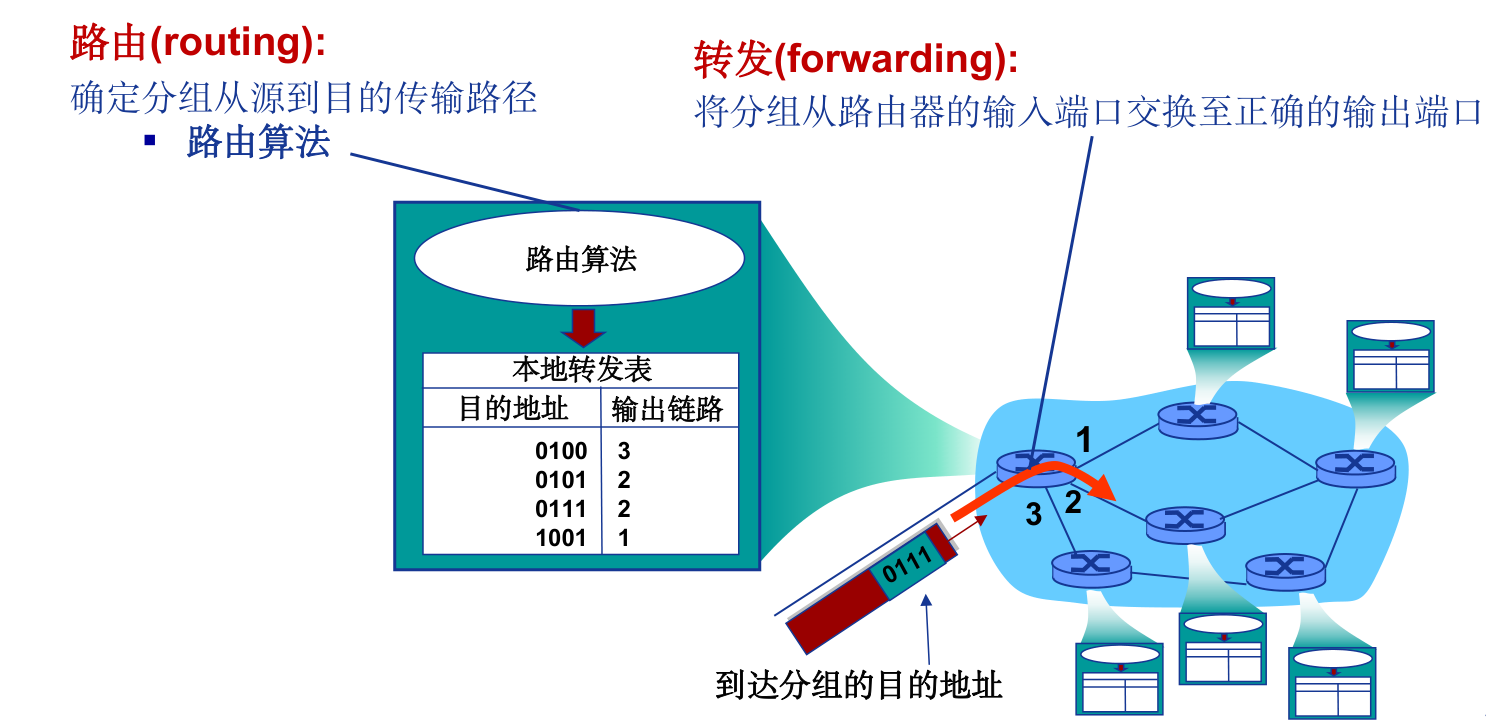
\includegraphics[width=0.82\textwidth]{ch01-routing-review.png}
  \caption{路由和转发的关系。左侧“路由算法”决定路径；右侧路由器按本地转发表把目的地址映射到输出链路。来源：\texttt{Chapter1-计算机网络概述.pdf}，PDF第31页（课件显示页31），局部截取。}
  \label{fig:ch01-routing-forwarding}
\end{figure}

\begin{quote}\small\textbf{来源：}课件\texttt{Chapter1-计算机网络概述.pdf}，PDF第31--32页（课件显示页31--32）；参考书第1章§1.1.2，PDF第13页／印刷第2页。\end{quote}
\annotationarea[4]

\subsection{Internet：网络之网络}

家庭、公司和大学等端系统通常先接入一个\textbf{接入ISP}（Internet Service Provider，互联网服务提供商）。接入ISP还必须继续互连，任意两个主机之间才可能交换分组。大量接入ISP若两两直接互连，网络规模增大时连接数量会急剧增加；对$N$个网络做完全两两连接需要$N(N-1)/2$条连接，数量级为$O(N^2)$。

课件用以下结构说明Internet中的互连关系：
\begin{itemize}
  \item 接入ISP可通过区域ISP连接到更大范围的网络。
  \item 不同ISP之间可通过对等链路（peering link）互连，也可在Internet交换点（IXP，Internet Exchange Point）交换流量。
  \item 少数一级（tier-1）商业ISP提供国家或国际范围的覆盖。
  \item 内容提供商网络（如课件列举的Google网络）可运行自己的网络，连接数据中心并就近提供服务。
\end{itemize}

课件强调Internet是不断演进的复杂“网络之网络”，没有单一、固定的结构图能精确表示所有互连关系。图\ref{fig:ch01-internet}是用于说明组成和关系的示意图。

\begin{quote}\small\textbf{来源：}课件\texttt{Chapter1-计算机网络概述.pdf}，PDF第33--41页（课件显示页33--41）。\end{quote}
\annotationarea[4]

\section{数据交换}

\subsection{为什么需要数据交换}

若每对主机都用一条专用链路直接互连，主机数量增多时，所需链路数量会迅速增加，而且链路资源难以共享。\textbf{交换网络}通过交换节点连接多台主机：数据进入网络后，由节点选择或使用相应链路送往目的端。课件将交换方式分为\textbf{电路交换、报文交换和分组交换}。

\begin{quote}\small\textbf{来源：}课件\texttt{Chapter1-计算机网络概述.pdf}，PDF第43--49页（课件显示页43--49）；参考书第1章§1.1.4，PDF第14--16页／印刷第3--5页。\end{quote}
\annotationarea[4]

\subsection{电路交换、报文交换与分组交换}

\begin{center}
\begin{tabularx}{0.98\textwidth}{l X X X}
\toprule
 & 电路交换 & 报文交换 & 分组交换\\
\midrule
传送单位 & 建立的端到端电路承载连续比特流 & 报文，即应用发送的信息整体 & 报文拆分得到的较小分组\\
开始发送前 & 先建立连接、占用资源 & 不需建立连接 & 不需建立连接\\
转发方式 & 建立电路后沿专用路径传输 & 节点完整接收一个报文后再转发 & 节点收到并存储分组后逐个转发\\
资源使用 & 通信期间独占所分配资源 & 报文传送时占用链路 & 分组传送时占用链路，可统计共享\\
结束时 & 释放连接和资源 & 无需拆除电路 & 无需拆除电路\\
\bottomrule
\end{tabularx}
\end{center}

\textbf{电路交换}最典型的例子是电话网络。其三个阶段是\textbf{建立连接（呼叫/电路建立）—通信—释放连接}。通信双方在数据传输前建立专用端到端通路，并在通信期间独占分配给该通路的资源。课件指出可用时分复用（TDM，Time-Division Multiplexing）或频分复用（FDM，Frequency-Division Multiplexing）让多路通信共享链路的不同时间片或频带；具体复用方式在物理层章节展开。

\textbf{报文交换}把源应用发送的信息整体作为一个报文，例如一个文件或一张图像。交换节点必须先完整接收并存储报文，再向下一跳转发。这会产生较大的存储转发等待，并要求节点能存下完整报文。

\textbf{分组交换}先把报文拆成较小的数据块，并在每块前添加首部等控制信息，形成分组；目的端再根据分组信息重组报文。拆装和添加首部会增加开销。节点按分组存储转发，不必等待整个报文到达后才开始转发，因此多个分组可以在不同链路上形成流水传输。

\textbf{统计多路复用（statistical multiplexing）}是分组交换共享链路的方式：有分组需要传送时才竞争使用链路，链路带宽不按用户永久切分。它适合突发数据并能提高资源共享程度；当到达流量超过链路和缓存的承受能力时，也可能出现分组排队、延迟和丢失。因此课件明确提出，分组交换并非在所有服务目标下都优于电路交换；需要带宽保障的音频或视频业务还要考虑性能保障机制。课件第74页提出“如何提供电路级性能保障”。\textbf{参考书补充（本课件未展开）：}若要在分组网络中承诺带宽，建立业务时应检查路径各链路是否有足够可用容量，并为获准业务预留资源；容量不足时拒绝接入或降低承诺。虚电路能固定转发路径，但路径固定本身不等于带宽预留；多个虚电路仍可共享链路。

\begin{quote}\small\textbf{来源：}课件\texttt{Chapter1-计算机网络概述.pdf}，PDF第46--58、73--74页（课件显示页相同）；参考书第1章§1.1.4，PDF第14--16页／印刷第3--5页；虚电路与数据报的差别见第4章§4.1.3，PDF第140--142页／印刷第129--131页。课件第53页将英文写作“package switching”；本笔记按课件中文术语“分组交换”书写。\end{quote}
\annotationarea[4]

\subsection{发送时延、存储转发和流水传输}

\textbf{发送时延（传输时延）}是把一个分组的全部比特推入链路所需的时间。设分组长$L$ bit、链路传输速率$R$ bit/s，则
\[
 t_{\mathrm{trans}}=\frac{L}{R}\quad(\mathrm{s}).
\]
此处$L$计量分组长度，$R$计量每秒可发送的比特数，结果单位是秒。它不是信号在链路中跑完距离所需的时间；传播时延将在性能部分定义。

对报文长度$M$ bit、分组长度$L$ bit、每条链路速率均为$R$的存储转发网络，若路径含$h$段链路（$n=h-1$个路由器），忽略传播、处理和排队时延，分组长度一致且$M$可被分组有效长度整除，则课件给出的流水传输完成时间为
\[
T=\frac{M}{R}+(h-1)\frac{L}{R}
 =\frac{M}{R}+n\frac{L}{R}.
\]
首项是源端发送全部数据所需时间；其余$h-1$项是末尾分组在中间路由器逐跳转发所增加的时间。该式解释了分组流水：第一个分组先经过各跳，后续分组可在前一分组已经进入下一链路时继续从源端发送。

\textbf{课件例题：报文交换与分组交换}（PDF第60--69页）。给定报文$M=7.5$ Mbit、分组长$L=1500$ bit、三段等速率链路$R=1.5$ Mbit/s，求报文从源端发送至目的端的时间，并比较交换节点所需的最小缓存。

\textbf{解：}
\begin{enumerate}
  \item 分组数为$M/L=7.5\times10^6/1500=5000$。
  \item 报文交换中，每个中间节点先接收整个报文。每段链路发送整个报文的时间是$M/R=7.5/1.5=5$ s；三段链路依次存储转发，总时间为$3\times5=15$ s。
  \item 分组交换中，单个分组的发送时延为$L/R=1500/(1.5\times10^6)=0.001$ s，即1 ms。课件图给出的流水完成时间为$5002$ ms，也可由$M/R+(3-1)L/R=5+0.002=5.002$ s得到。
  \item 若问题问“至少要能存下一个完整的待转发单位”，报文交换节点需能存下整个报文$M=7.5$ Mbit；分组交换节点需能存下一个完整分组$L=1500$ bit。实际队列总缓存大小还取决于同时排队的分组数量，课件数据不足以计算该总量。
\end{enumerate}
\annotationarea[4]

\begin{quote}\small\textbf{来源：}课件\texttt{Chapter1-计算机网络概述.pdf}，PDF第59--70页（课件显示页59--70）；参考书第1章§1.1.4，PDF第15--16页／印刷第4--5页。\end{quote}
\annotationarea[4]

\subsection{课件例题1：文件经两台路由器传送}

\textbf{题目}（课件例1，PDF第71页）：采用存储转发的分组交换网络中，所有链路速率为100 Mb/s。每个分组总长1000 B，分组头20 B。主机$H_1$向$H_2$发送980000 B文件，路径经过两个路由器。忽略分组拆装时间和传播时延，求从$H_1$开始发送到$H_2$接收完所需的最短时间。

\textbf{解：}每个分组可承载的文件数据为$1000-20=980$ B，因此分组数为$980000/980=1000$。每个分组在线路上仍占1000 B，故$H_1$发送完全部分组需要
\[
 t_{H_1}=\frac{1000\times1000\times8}{100\times10^6}\ \mathrm{s}
 =0.080\ \mathrm{s}=80\ \mathrm{ms}.
\]
在速率相同的链路上，分组流水传输时，最后一个分组还要经过两个路由器转发；增加的时间为
\[
 t_{\mathrm{extra}}=2\times\frac{1000\times8}{100\times10^6}\ \mathrm{s}
 =0.00016\ \mathrm{s}=0.16\ \mathrm{ms}.
\]
所以$H_2$接收完整个文件至少需$80+0.16=80.16$ ms。这里计算的是分组总长（含分组头）的链路占用时间；忽略题目明确排除的拆装和传播时间。
\annotationarea[4]

\begin{quote}\small\textbf{来源：}课件\texttt{Chapter1-计算机网络概述.pdf}，PDF第71--72页（课件显示页71--72）；参考书第1章§1.1.4同类存储转发计算，PDF第15--16页／印刷第4--5页。\end{quote}
\annotationarea[4]

\subsection{课件例题：分组交换与电路交换的资源共享}

\textbf{题目}（课件PDF第73页）：一条1 Mb/s链路上，每个用户活动时需100 kb/s，平均活动时间占10\%。电路交换可支持多少用户？35个用户使用分组交换时，超过10人同时活动的概率是多少？

\textbf{解：}电路交换需要为每个用户预留100 kb/s，因此$1$ Mb/s$/100$ kb/s$=10$个用户。分组交换不为每位用户永久预留全部活动速率；若额外假设各用户是否活动相互独立，令同时活动人数为随机变量$X$，则$X$服从参数$n=35,p=0.1$的二项分布。超过10人同时活动的概率为
\[
\Pr(X>10)=\sum_{k=11}^{35}{35\choose k}(0.1)^k(0.9)^{35-k}
\approx 0.0004243.
\]
该数约为$4.24\times10^{-4}$。课件写作“$<0.0004$”；按上述独立二项模型精算，该严格不等式不成立，$0.0004243$可粗略写成$0.0004$（保留一位有效数字）。课件未明说独立性，这是计算该概率所需的建模前提。分组交换因用户并非总在活动，可让更多用户共享链路，但超过链路能力时仍会排队或丢包。
\annotationarea[4]

\begin{quote}\small\textbf{来源与核对：}课件\texttt{Chapter1-计算机网络概述.pdf}，PDF第73--74页（课件显示页73--74）。课件给出“$<0.0004$”；按独立活动假设求二项分布尾概率为约$0.0004243$，故这里保留课件数值并说明精算差异。\end{quote}
\annotationarea[4]

\section{计算机网络性能指标}

\subsection{速率、带宽与吞吐量}

\textbf{速率}即数据率或比特率，表示单位时间传输的数据量，是课件列出的重要性能指标。课件此处按十进制使用$1$ kb/s$=10^3$ bit/s、$1$ Mb/s$=10^6$ bit/s、$1$ Gb/s$=10^9$ bit/s、$1$ Tb/s$=10^{12}$ bit/s。课件还指出，速率往往指额定或标称速率。注意bit（比特）与B（字节）不同：$1$ B$=8$ bit。网络语境下“带宽”常指数字信道可传送的最高数据率，单位为bit/s；信号语境中的频带宽度是最高频率与最低频率之差，单位为Hz，两种语境不可混用。

\textbf{吞吐量（throughput）}是发送端与接收端之间实际传送数据的速率。\textbf{即时吞吐量}描述某一时刻的速率；\textbf{平均吞吐量}是在一段时间内平均得到的速率。路径上的链路速率可能不同，端到端吞吐量受瓶颈链路限制。若服务器侧速率为$R_s$、客户侧速率为$R_c$，且路径中间链路速率为$R$并由10条连接平均共享，课件给出的每条连接吞吐量为
\[
\min(R_c,R_s,R/10).
\]
\textbf{课件提示题：}若$R_s<R_c$，端到端吞吐量受$R_s$限制；若$R_s>R_c$，则受$R_c$限制。共同原则是取端到端路径中可用速率的最小值。

\begin{quote}\small\textbf{来源：}课件\texttt{Chapter1-计算机网络概述.pdf}，PDF第77--78、88--90页（课件显示页77--78、88--90）；参考书第1章§1.1.5，PDF第17--19页／印刷第6--8页。\end{quote}
\annotationarea[4]

\subsection{结点时延与分组丢失}

分组经过结点时会经历四类时延。设分组长$L$ bit、输出链路速率$R$ bit/s、链路长度$d$ m、信号传播速度$s$ m/s，则
\[
\begin{aligned}
 d_{\mathrm{nodal}}&=d_{\mathrm{proc}}+d_{\mathrm{queue}}+d_{\mathrm{trans}}+d_{\mathrm{prop}},\\
 d_{\mathrm{trans}}&=\frac{L}{R},\qquad
 d_{\mathrm{prop}}=\frac{d}{s}.
\end{aligned}
\]
各量的含义如下：
\begin{itemize}
  \item \textbf{处理时延}$d_{\mathrm{proc}}$：结点检查分组首部、进行差错检测、确定输出端口等处理所需的时间。课件指出通常小于毫秒。
  \item \textbf{排队时延}$d_{\mathrm{queue}}$：分组在输出队列中等待链路可用的时间，取决于到达流量和队列状态。
  \item \textbf{发送时延}$d_{\mathrm{trans}}$：把分组全部比特发送到链路上所需时间。它由分组长度和链路速率决定。
  \item \textbf{传播时延}$d_{\mathrm{prop}}$：信号沿物理介质传播所需时间。它由链路长度和介质中的传播速度决定。
\end{itemize}

课件以$2\times10^8$ m/s作为链路信号传播速度的近似值。\textbf{发送时延和传播时延不是一回事：}增大速率$R$会缩短发送时延；缩短距离$d$或提高传播速度$s$会缩短传播时延。处理与排队则发生在结点。

\begin{figure}[H]
  \centering
  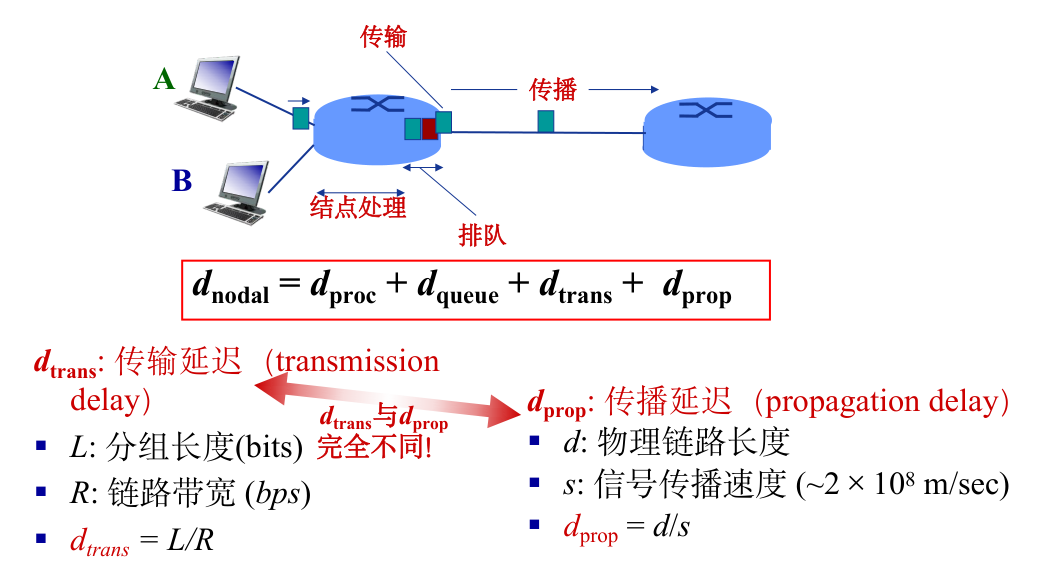
\includegraphics[width=0.82\textwidth]{ch01-delay.png}
  \caption{结点的四类时延及其合成关系。图中$d_{\mathrm{trans}}$表示把整包比特送入链路的过程，$d_{\mathrm{prop}}$表示信号在链路中传播的过程。来源：\texttt{Chapter1-计算机网络概述.pdf}，PDF第81页（课件显示页81），局部截取。}
  \label{fig:ch01-delay}
\end{figure}

\textbf{排队流量强度}用于描述分组到达速率与链路服务能力的关系。令$a$为平均分组到达速率（packet/s），$L$为平均分组长度（bit），$R$为链路速率（bit/s），则
\[
\rho=\frac{La}{R}.
\]
$La$是平均到达的比特速率。课件指出：$\rho$接近0时平均排队时延很小；$\rho$接近1时平均排队时延会很大；$\rho>1$时到达速率超过链路处理能力，在理想无限队列模型下平均排队时延发散，实际有限队列会导致丢包。

课件用车队类比区分发送与传播：收费站放行一辆车所需时间对应发送一个比特的时间；车队中每辆车对应一个比特，整队通过收费站所需时间对应分组发送时延；车从一个收费站行驶到下一个收费站的时间对应传播时延。课件例子中车队由10辆车组成、每辆放行需12秒，整队通过需120秒；两站相距100 km、车速100 km/h，单车到下一站需1小时。这个类比表明，队列整体通过服务点的时间与每个车/比特在路径上行进的时间是两种不同量。

\textbf{分组丢失（丢包）}：路由器队列缓存容量有限；如果新分组到达时队列已满，该分组可能被丢弃。丢弃的分组可能由前序结点或源端重发，也可能不重发。课件定义
\[
\text{丢包率}=\frac{\text{丢包数}}{\text{已发送分组总数}}.
\]

\begin{quote}\small\textbf{来源：}课件\texttt{Chapter1-计算机网络概述.pdf}，PDF第79--83、87页（课件显示页79--83、87）；参考书第1章§1.1.5，PDF第18--19页／印刷第7--8页。\end{quote}
\annotationarea[4]

\subsection{时延带宽积、往返时间和利用率}

若传播时延为$d_{\mathrm{prop}}$、链路速率为$R$ bit/s，\textbf{时延带宽积}为
\[
  d_{\mathrm{prop}}R\quad(\text{bit}).
\]
它表示信号传播期间，链路中能够容纳的比特数量；单位是bit。课件把它称为“以比特为单位的链路长度”。

\textbf{往返时间（RTT，Round-Trip Time）}的口径在不同材料中不同。课件第85页把RTT定义为从发送方发送完数据到开始收到确认数据所经历的时间；ACK（acknowledgment，确认）是接收方发回的确认分组。课件用简化式
\[
\mathrm{RTT}=t_P+t_{\mathrm{PRC}}+t_P=2t_P+t_{\mathrm{PRC}}
\]
表示：$t_P$是单向传播时延，$t_{\mathrm{PRC}}$是接收方处理时延；此简化式未计中间结点时延。课件接着写出响应时间
\[
T_{\mathrm{response}}=t_{\mathrm{PKT}}+\mathrm{RTT}+t_{\mathrm{ACK}},
\]
其中$t_{\mathrm{PKT}}$、$t_{\mathrm{ACK}}$分别表示数据分组和确认分组的发送时延。

参考书对RTT的定义是：从发送端发出一个短分组到收到接收端确认所经历的时间；包含往返传播时延、接收端处理时延以及互联网中间节点的处理和排队时延，但不包括数据分组本身的发送时延（参考书第1章§1.1.5，PDF第19页／印刷第8页）。实际题目须按题目或课件给定口径判断是否计入发送、排队及中间处理时延；本章课堂公式以PPT的简化口径为主。

\textbf{信道利用率}是信道被使用的时间占总时间的比例；课件把\textbf{网络利用率}定义为全网络各信道利用率的加权平均。课件第86页停等图的公式图像存在疑似笔误：分子是$t_{\mathrm{PKT}}$，但分母显示为$t_{\mathrm{ACK}}+\mathrm{RTT}+t_{\mathrm{ACK}}$；这与相邻第85页的响应时间表达式不一致。若用“发送数据分组的时间/一个完整发送周期”计算停等发送方利用率，且周期由数据发送、RTT和ACK发送组成，则一致的计算式应为
\[
U=\frac{t_{\mathrm{PKT}}}{t_{\mathrm{PKT}}+\mathrm{RTT}+t_{\mathrm{ACK}}}.
\]
这里将课件疑似笔误明确标出，不能把第86页图上分母原样当作正确结果。不同教材可能对利用率、响应时间和RTT的计时起点作不同约定，计算时应先列出一个周期所包含的事件。

\begin{figure}[H]
  \centering
  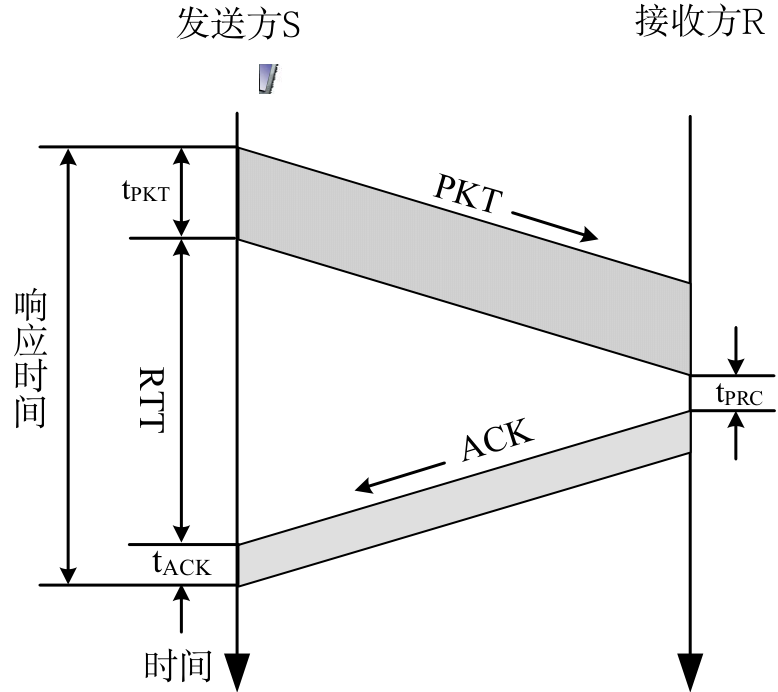
\includegraphics[width=0.80\textwidth]{ch01-rtt-review.png}
  \caption{课件的RTT与响应时间示意。数据分组由S发往R，R处理后返回ACK；图中$t_{\mathrm{PKT}}$和$t_{\mathrm{ACK}}$是发送时间，斜向传播段体现传播时间。来源：\texttt{Chapter1-计算机网络概述.pdf}，PDF第85页（课件显示页85），局部截取。}
  \label{fig:ch01-rtt}
\end{figure}

\begin{quote}\small\textbf{来源与核对：}课件\texttt{Chapter1-计算机网络概述.pdf}，PDF第84--86页（课件显示页84--86）；参考书第1章§1.1.5，PDF第19--20页／印刷第8--9页。PPT与参考书的RTT定义范围不同；PPT第86页利用率公式分母与第85页响应时间式不一致，正文按事件周期给出一致式并保留差异说明。\end{quote}
\annotationarea[4]

\subsection{课件例题2：吞吐量、完成时间与路由器排队}

\textbf{题目}（课件例2，PDF第91页）：主机A经路由器R1、R2连接主机B，A以存储转发方式发送大文件。课件文字给出的三段链路速率依次为100 kb/s、2 Mb/s和1 Mb/s。求无其他流量时最大吞吐量；文件为4 MB时的传输时间；分组是否排队以及排队位置。

\textbf{（1）最大吞吐量。} 端到端吞吐量由最慢链路限制：
\[
\min(100\ \mathrm{kb/s},2\ \mathrm{Mb/s},1\ \mathrm{Mb/s})=100\ \mathrm{kb/s}.
\]

\textbf{（2）文件传输时间。} 课件注释$1$ k$=10^3$、$1$ M$=10^6$，因此$4$ MB$=4\times10^6$ B$=32\times10^6$ bit。按瓶颈吞吐量估算，
\[
T=\frac{32\times10^6\ \mathrm{bit}}{100\times10^3\ \mathrm{bit/s}}=320\ \mathrm{s}.
\]
该估算适用于大文件稳态传输并忽略起始流水填充等附加时间，符合课件给出的近似题意。

\textbf{（3）排队位置及资料冲突。} 课件第91页文字按A至B顺序写100 kb/s、2 Mb/s、1 Mb/s；但同页网络图及第94页排队图画的是1 Mb/s、2 Mb/s、100 kb/s。图示局部如下：
\begin{figure}[H]
  \centering
  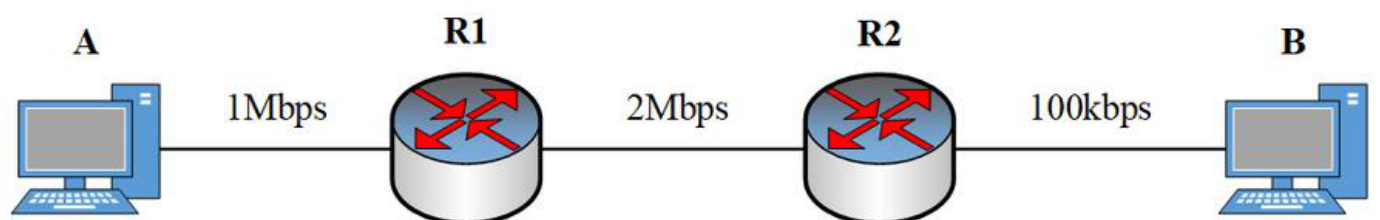
\includegraphics[width=0.80\textwidth]{ch01-throughput-example.png}
  \caption{课件例2的链路速率图。按图示方向，A--R1为1 Mb/s、R1--R2为2 Mb/s、R2--B为100 kb/s。来源：\texttt{Chapter1-计算机网络概述.pdf}，PDF第91页（课件显示页91），局部截取。}
  \label{fig:ch01-throughput-example}
\end{figure}
按图示顺序，分组到达R2的速度快于R2向100 kb/s末段链路发送的速度，故持续发送时会在R2输出队列排队；这与课件第94页给出的“在R2发生排队”相符。若按第91页文字顺序理解，即第一段已是100 kb/s、后续链路更快，则持续分组的到达间隔由慢速第一段决定，后续链路能更快服务，不会因这三段速率关系在R1或R2形成持续排队。两种读法的瓶颈吞吐量和大文件近似时间相同，但排队位置结论不同；本笔记保留这一处课件图文冲突，不把图和文字混用。
\annotationarea[4]

\begin{quote}\small\textbf{来源与核对：}课件\texttt{Chapter1-计算机网络概述.pdf}，PDF第91--94页（课件显示页91--94）。第91页文字与网络图的速率顺序不一致；第94页“在R2排队”的答案与图示顺序相符。参考书第1章§1.1.5关于瓶颈链路的说明，PDF第19页／印刷第8页。\end{quote}
\annotationarea[4]

\section{计算机网络体系结构}

\subsection{分层结构、实体、协议、服务与接口}

计算机网络涉及主机、路由器、链路、应用、协议、硬件和软件等大量部分。\textbf{分层结构}把复杂系统拆成若干层，每层完成一类功能，使用下层提供的服务，并向上层提供服务。分层有助于描述系统、模块化设计、维护更新和标准化；改变某层的实现时，只要其服务约定不变，上下层通常不必了解其内部实现。

\textbf{网络体系结构}是计算机网络各层及其协议的集合，是从功能角度描述网络层次及其相互关系的抽象结构。层次模型规定功能边界，不等同于具体设备中软件和硬件模块的唯一划分。

课件指出分层使结构清晰、便于模块更新维护，并有利于标准化；同时在第99页提出“分层是否有不利之处”但未直接作答。结合课件第105页说明的封装过程可知，逐层添加控制信息会增加传输开销；课件没有在本章系统展开其他缺点。

课件第100页给出以下基本概念：
\begin{itemize}
  \item \textbf{实体（entity）}：任何可发送或接收信息的硬件或软件进程。
  \item \textbf{对等实体}：位于不同系统、处于相同层次并按同层协议通信的实体。它们遵循的协议是逻辑上“水平”的。
  \item \textbf{服务}：某层向其上一层提供的功能。服务使用关系是相邻层之间“垂直”的；上层使用服务，不必了解下层如何实现。
  \item \textbf{接口}：同一系统中相邻层实体交换信息的边界。
  \item \textbf{服务访问点（SAP，Service Access Point）}：上层实体访问下层服务的位置；双方通过服务原语请求或使用特定服务。
\end{itemize}

\begin{figure}[H]
  \centering
  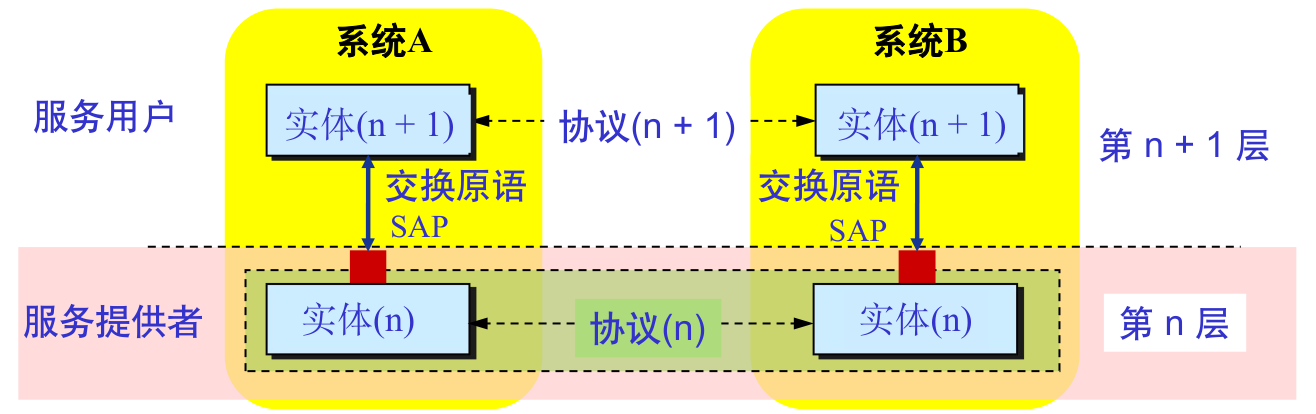
\includegraphics[width=0.82\textwidth]{ch01-layer-services-review.png}
  \caption{对等协议、层间服务和SAP。左右系统中同层实体按协议交换信息；每个系统内部由下层向相邻上层提供服务，SAP是服务访问位置。来源：\texttt{Chapter1-计算机网络概述.pdf}，PDF第100页（课件显示页100），局部截取。}
  \label{fig:ch01-layer-service}
\end{figure}

\textbf{协议数据单元（PDU）}是某层按本层协议处理和交换的数据单位。封装时，下层在上层数据外加入本层需要的控制信息，例如标识发送端或接收端的地址、用于差错检测或纠正的编码，以及实现协议功能的控制信息（如优先级、服务质量和安全控制）。PPT第105页将这些控制信息作为构造PDU的原因。

\begin{quote}\small\textbf{来源：}课件\texttt{Chapter1-计算机网络概述.pdf}，PDF第96--100、104--105页（课件显示页96--100、104--105）；参考书第1章§1.2.1，PDF第26--29页／印刷第15--18页。\end{quote}
\annotationarea[4]

\subsection{OSI七层参考模型及各层功能}

国际标准化组织（ISO）于1984年提出\textbf{开放系统互连（OSI）参考模型}，用于描述异构系统怎样互连。它是理解网络通信的理论模型，课件指出“理论成功，市场失败”。OSI自下而上共七层：

\begin{center}
\begin{tabularx}{0.98\textwidth}{c l X}
\toprule
层号 & 层名 & 课件所列主要功能\\
\midrule
7 & 应用层 & 为用户程序提供网络服务；例：HTTP、FTP、SMTP。\\
6 & 表示层 & 处理信息表示的语法和语义；可进行主机无关格式转换、编码、加密/解密、压缩/解压缩。\\
5 & 会话层 & 管理对话；建立和维护会话；在数据流中插入同步点。\\
4 & 传输层 & 提供源到目的端的进程间完整报文传输；分段与重组、SAP寻址、连接控制、流量控制和差错控制。\\
3 & 网络层 & 负责源主机到目的主机的分组传送，可能穿越多个网络；逻辑寻址（例如IP地址）、路由和转发。\\
2 & 数据链路层 & 负责相邻结点间传输；组帧、物理寻址、流量控制、差错控制、介质访问控制。\\
1 & 物理层 & 在物理介质上发送比特；规定接口特性、比特编码、数据率、时钟同步和传输模式：单工只单向传输，半双工双方轮流，全双工双方可同时传输。\\
\bottomrule
\end{tabularx}
\end{center}

\textbf{按通信范围辨别层次：}数据链路层处理相邻结点之间的传输；网络层把分组从源主机送到目的主机，可能经过多个网络；传输层面向不同主机上的应用进程，处理端到端传输。应用层与用户可见的网络服务相邻。课件列出的数据链路层差错控制和传输层差错控制处于不同通信范围，不应混为一个功能。

数据链路层的流量控制用于避免发送方“淹没”接收方；差错控制用于检测损坏或丢失帧，并可重传、避免重复帧；介质访问控制用于决定共享链路在给定时刻由哪个设备使用。传输层的SAP寻址要把完整报文交给正确进程，课件以端口号为例；分段与重组、连接控制、流量控制和差错控制面向源到目的的进程通信。

\textbf{数据封装}发生在发送端：上层数据逐层向下交付，各层根据协议加入本层控制信息，形成相应PDU；接收端逐层向上处理并移除对应控制信息。传输过程中，中间系统只需实现转发所需的层次，不必像端系统那样处理全部应用层功能。

\begin{quote}\small\textbf{来源：}课件\texttt{Chapter1-计算机网络概述.pdf}，PDF第101--115页（课件显示页101--115）；参考书第1章§1.2.2，PDF第29--34页／印刷第18--23页。\end{quote}
\annotationarea[4]

\subsection{TCP/IP模型与五层参考模型}

课件给出的\textbf{TCP/IP（传输控制协议/网际协议）模型}自上而下为\textbf{应用层、传输层、网际层、网络接口层}。网络接口层连接具体网络技术；网际层中的IP为不同应用和网络提供互联服务。课件用“Everything over IP”和“IP over Everything”概括：IP可为各种应用提供服务，也可运行在多种网络技术之上。

用于学习网络通信过程时，课件还介绍综合OSI和TCP/IP模型优点的\textbf{五层参考模型}：
\begin{itemize}
  \item \textbf{应用层}：支持网络应用，如FTP（文件传输协议）、SMTP（Simple Mail Transfer Protocol，简单邮件传输协议）、HTTP（超文本传输协议）。
  \item \textbf{传输层}：负责进程到进程的数据传输，如TCP和UDP（User Datagram Protocol，用户数据报协议）。
  \item \textbf{网络层}：负责源主机到目的主机的分组传送、路由和转发，如IP。
  \item \textbf{数据链路层}：负责相邻网络元素之间的数据传输，如以太网、802.11（Wi-Fi）和PPP。
  \item \textbf{物理层}：负责比特传输。
\end{itemize}

\textbf{五层模型的PDU名称}按课件第119页为：应用层\textbf{报文（message）}，传输层\textbf{段（segment）}，网络层\textbf{数据报（datagram）}，数据链路层\textbf{帧（frame）}，物理层传送\textbf{比特（bits）}。封装时每层加入本层首部等信息；路由器按课件图处理到网络层并在相邻链路上重新封装帧，交换机处理数据链路层和物理层；端系统运行完整五层模型。

\begin{figure}[H]
  \centering
  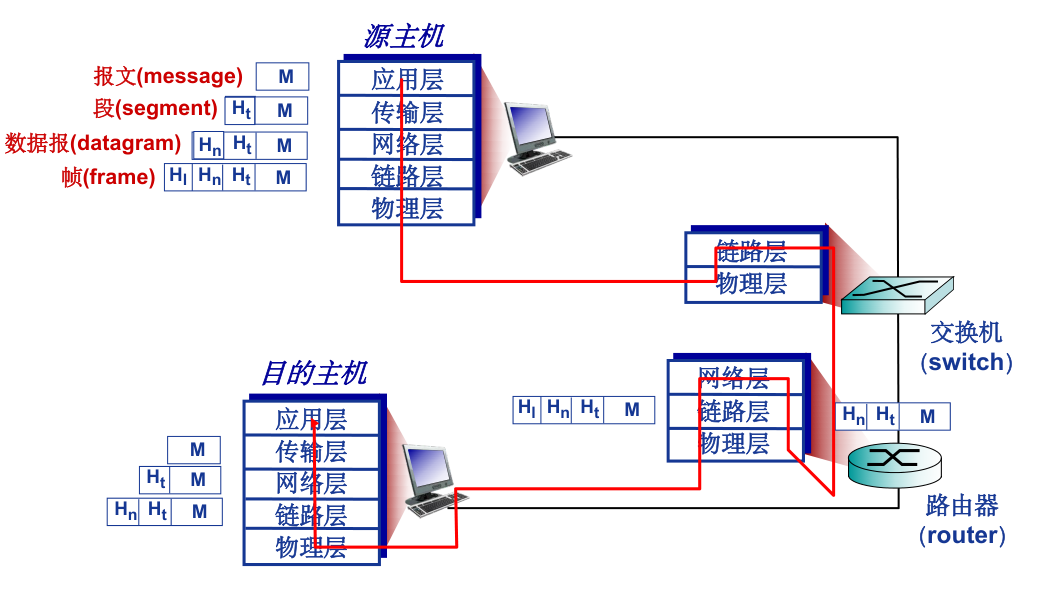
\includegraphics[width=0.84\textwidth]{ch01-encapsulation.png}
  \caption{五层模型下的封装与中间设备处理范围。应用数据逐层加入首部成为段、数据报和帧，最终变成比特；路由器转发网络层数据，交换机按链路层信息转发帧。来源：\texttt{Chapter1-计算机网络概述.pdf}，PDF第119页（课件显示页119），局部截取。}
  \label{fig:ch01-encapsulation}
\end{figure}

\begin{quote}\small\textbf{来源：}课件\texttt{Chapter1-计算机网络概述.pdf}，PDF第116--119页（课件显示页116--119）；参考书第1章§1.2.2，PDF第34--38页／印刷第23--27页。\end{quote}
\annotationarea[2]

\section{计算机网络发展历史（课件标注“略”）}

\subsection{课件时间线}

本节按课件列出的里程碑整理，课件第120页将其标注为“略”。年份和事件是帮助识别发展阶段的时间线，不替代各协议的后续章节。

\begin{center}\small
\begin{tabularx}{0.96\textwidth}{l X}
\toprule
时期 & 课件列出的事件\\
\midrule
1961--1972 & 1961年Kleinrock用排队论分析分组交换有效性；1964年Baran研究分组交换在军事网络中的应用；1967年美国高级研究计划局（ARPA，Advanced Research Projects Agency）提出ARPAnet构想；1969年首个ARPAnet结点运行。1972年ARPAnet公开演示，出现第一个主机到主机协议NCP（Network Control Protocol，网络控制协议）和第一个电子邮件程序，ARPAnet有15个结点。\\
1972--1980 & 1970年ALOHA卫星网络建成；1974年Cerf与Kahn提出网络互连体系结构；1975年ARPAnet移交美国国防部通信局管理；1976年Xerox设计以太网；20世纪70年代后期出现DECnet、SNA、XNA等私有体系结构及固定长度分组交换（ATM，异步传递模式的先驱）；1979年ARPAnet有200个结点。课件概括的互连原则包括极简、自治、尽力服务、无状态路由器和分散控制。\\
1980--1990 & 1982年定义SMTP（Simple Mail Transfer Protocol，简单邮件传输协议）；1983年部署TCP/IP并定义DNS（Domain Name System，域名系统）；1985年定义FTP；1986年美国国家科学基金会网络（NSFnet）形成骨干网、区域网和校园网组成的三级网络；1988年出现TCP拥塞控制。课件还列出CSnet、BITnet、NSFnet、Minitel等新型网络，以及当时约10万台主机连接公共网络。\\
1990--2000年代 & 20世纪90年代初ARPAnet退役；1991年NSF解除NSFnet商业应用限制，NSFnet于1995年退役并由私营企业经营；1992年Internet Society（ISOC，互联网协会）成立。Web依托超文本（Bush于1945年、Nelson于20世纪60年代提出相关思想）、HTML和HTTP发展；1994年出现Mosaic和Netscape浏览器，90年代后期Web开始商业应用。课件还列出即时消息、P2P文件共享、网络安全、主机约5万和用户逾1亿等历史数据，以及Gb/s级网络主干。\\
2005年至今（按课件表述） & 宽带接入和高速无线接入增长；课件列出约50亿台移动终端（2016年）和38.9亿互联网用户（2018年）等当时统计；社交网络发展，课件列举Facebook用户很快达到10亿；Google、Microsoft等服务提供商建设专用网络；电子商务、大学和企业把服务运行在Amazon EC2、Azure等云平台中。上述数字仅是课件所列历史统计，不代表当前数据。\\
\bottomrule
\end{tabularx}
\end{center}

\begin{quote}\small\textbf{来源：}课件\texttt{Chapter1-计算机网络概述.pdf}，PDF第120--125页（课件显示页120--125）；其中第120页标题明确标注“略”。\end{quote}

